\section{A numerical example}\label{sec:numerical}
\begin{itemize}
    \item Introduce example problem (target = sol to forward/primal eqn with a known source/forcing $g$)
    \item Convergence plots (both "iterative" error $u^{(k)} - u^{(k-1)}$ and "absolute" error $u^{(k)}-u^{(*)}$)
    \item Plots showing comparison of target sol and actual obtained sol (snapshots in time) ((Maybe not))
    \item Example sol of forward equation using Monte Carlo
    \item Example sol of backward equation? Maybe.
\end{itemize}

In this section, we introduce a simple test case for testing out the proposed numerical method. We plot the error as a function of number of iterations $k$, and see a numerical indication of the convergence of the scheme, both in terms of the difference between successive iterates of $u^{(k)}$ and $z^{(k)}$, and in terms of the difference between $u^{(k)}$ and the target $d_T$.

\subsection{Setting for numerical results}
For the purposes of numerical simulations, we consider a simple Gaussian target radiation intensity given by
%
\begin{align}
    d_T(t,x,v) = \exp\Big[ -c\big( {(x-e)}^2 + {(v-d)}^2 \big) \Big].
\end{align}
%
Additionally, we fix the initial condition $u(0,x,v)$ to be 
%
\begin{align}
    f_0(x,v) = \exp\Big[ -c\big( {(x-e)}^2 + {(v-d)}^2 \big) \Big].
\end{align}
%
We note that this choice means that the target $d_T$ and the actual radiation intensity $u^{(k)}(t,x,v)$ will always coincide at the initial time $t=0$. 

In terms of parameters for the numerical simulations, we consider a solution domain $[0,T]\cross \Omega = [0,1]\cross[0,1]\cross[0,1]$, and a grid consisting of $N=20$ interior points in time, and $M=20$ interior points in $x$ and $v$ respectively. For the Monte Carlo simulations, we keep the same discretisation grid in $(t,x,v)$, and run $M_{MC}=400$ Monte Carlo simulations for each gridpoint. We fix the regularisation parameter $\alpha=4$, and run $K=20$ iterations, where each iteration consists of solving for the primal equation and the dual equation once, obtaining $u^{(k)}$ and $z^{(k)}$.

\subsection{Numerical results}

We define the iterative error as
%
\begin{align} 
    e_{IT}(k) := \lVert u^{(k)}-u^{(k-1)} \rVert^2_{L^2([0,T],L^2(\Omega))}
\end{align}
%
for $u$, and similarly for $z$. Numerically, we compute the difference between the discretised, numerical approximation of $u^{(k)}$ and that of $u^{(k-1)}$, and sum up the squared difference across all gridpoints, before normalising by dividing by the total number of points on the grid. In other words, we compute the mean squared error.

We similarly define the absolute error as 
%
\begin{align} 
    e_{ABS}(k) := \lVert u^{(k)}-d_T \rVert^2_{L^2([0,T],L^2(\Omega))},
\end{align}
%
and compute it across the discretisation grid as the mean squared error, in the same way as the iterative error. We choose to compute the error in the $L^2([0,T],L^(\Omega))$-norm, since this is the norm in which we chose to formulate the optimisation problem described in \autoref{eq:to-minimise}. 

\begin{figure}[h]
    \centering
    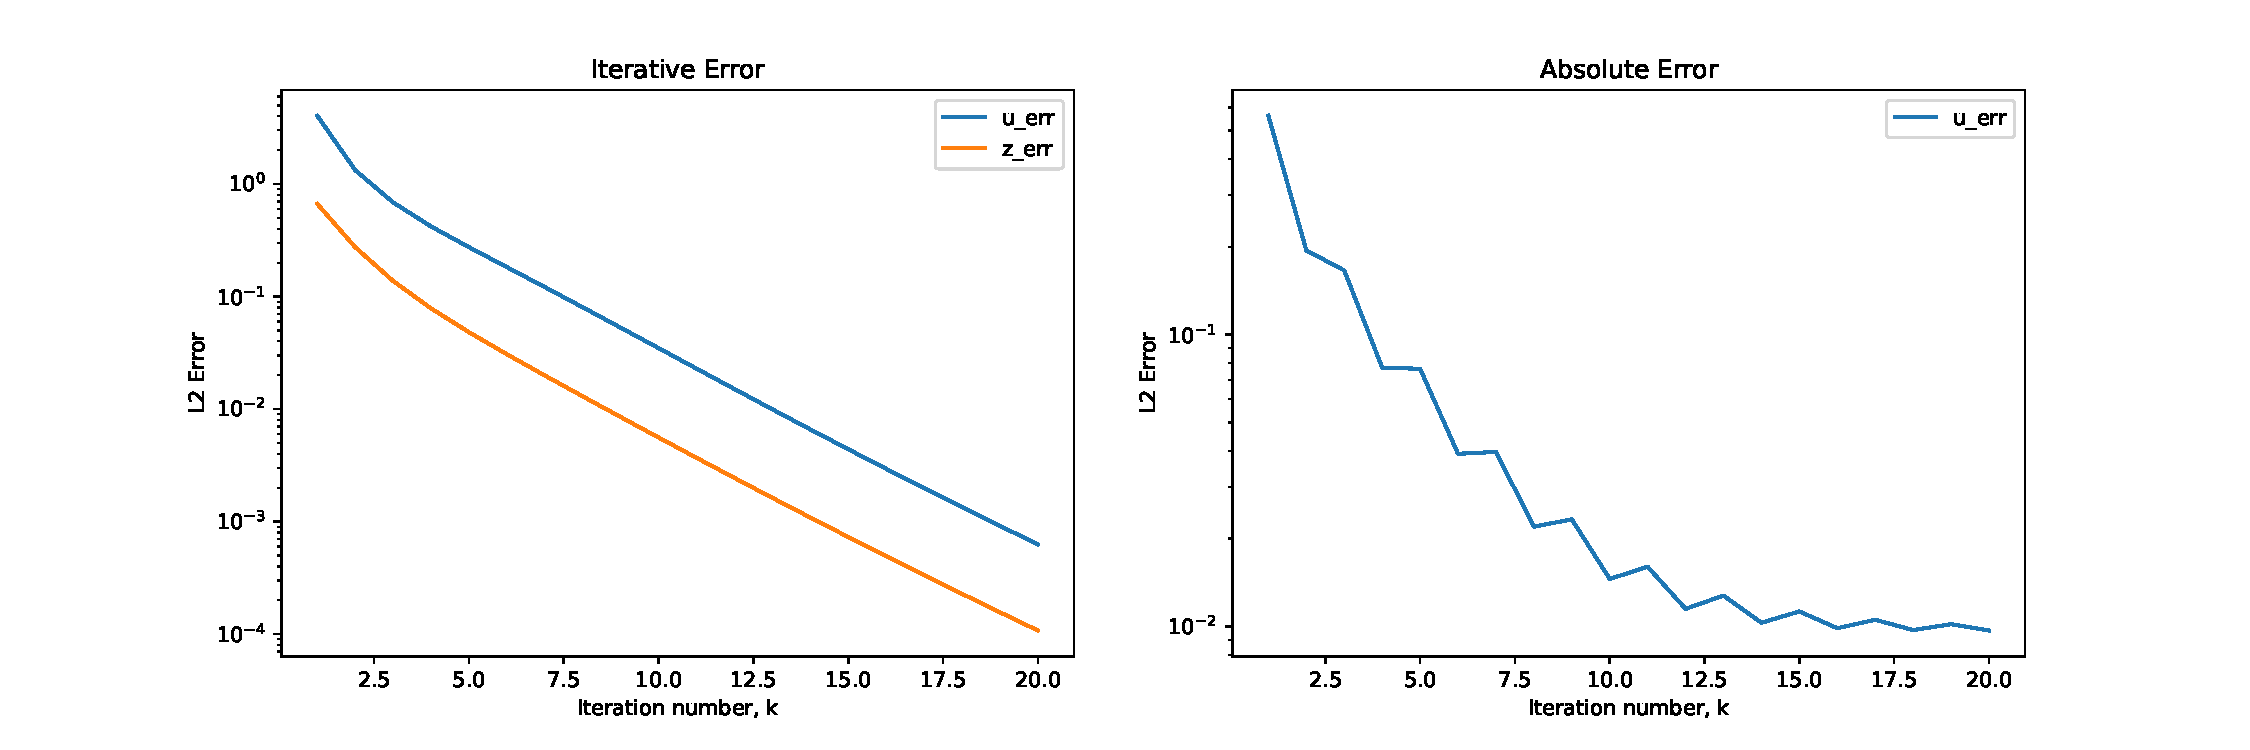
\includegraphics[width=0.9\textwidth]{error_plots.pdf}
    \caption{Error plots, showing error in the $L^2([0,T],L^2(\Omega))$-norm. Left: the error between successive iterates $u^{(k)}-u^{(k-1)}$ and $z^{(k)}-z^{(k-1)}$. Right: the error between $u^{(k)}$, the current iterate, and the target $d_T$.}\label{fig:error-plots}
\end{figure}

In \autoref{fig:error-plots} we plot the iterative and absolute errors, $e_{IT}(k)$ and $e_{ABS}(k)$ versus the iteration number $k$. Both errors are plotted on a log-linear scale. We see that the iterative error looks like a straight line on this scale, which implies that convergence occurs in terms of a power law, i.e. that the error is proportional to $k^{n}$, for some number $n$. Meanwhile, the absolute error is not a straight line on the log-linear scale. Instead, it looks to be decreasing faster than linearly on average, but it's decreasing in a very jagged fashion, decreasing a lot more over one iteration in some cases than others, and possibly even increasing slightly over one iteration in some cases. For later iterations, the absolute error seems to converge to a value of the order of $10^{-2}$. 

We note that depending on the choice of $d_T$, in general the sought-after minimum might not, even in theory, be $u=d_T$. This could explain the fact that the absolute error does not seem to go to zero. An additional explanation could be that due to discretisation error, the values of the "true" optimum of the discretised optimisation problem and the values of the target function $d_T$ on the grid, will not be exactly equal for any finite discretisation. 

In this report, we have not gone into detail on the difference between the non-discretised optimisation problem and the discretised optimisation problem. In the field of PDE constrained optimisation, a distinction is often made between choosing to optimise (and thus, if the Lagrangian method is chosen, derive the coupled PDE system) first, and then discretising to solve the system numerically, or instead discretising first, and then optimising the discretised problem. For an in-detail discussion of this distinction, see e.g. \cite{rees_preconditioning_2010}. 
